\documentclass[twoside]{book}

% Packages required by doxygen
\usepackage{fixltx2e}
\usepackage{calc}
\usepackage{doxygen}
\usepackage[export]{adjustbox} % also loads graphicx
\usepackage{graphicx}
\usepackage[utf8]{inputenc}
\usepackage{makeidx}
\usepackage{multicol}
\usepackage{multirow}
\PassOptionsToPackage{warn}{textcomp}
\usepackage{textcomp}
\usepackage[nointegrals]{wasysym}
\usepackage[table]{xcolor}

% Font selection
\usepackage[T1]{fontenc}
\usepackage[scaled=.90]{helvet}
\usepackage{courier}
\usepackage{amssymb}
\usepackage{sectsty}
\renewcommand{\familydefault}{\sfdefault}
\allsectionsfont{%
  \fontseries{bc}\selectfont%
  \color{darkgray}%
}
\renewcommand{\DoxyLabelFont}{%
  \fontseries{bc}\selectfont%
  \color{darkgray}%
}
\newcommand{\+}{\discretionary{\mbox{\scriptsize$\hookleftarrow$}}{}{}}

% Page & text layout
\usepackage{geometry}
\geometry{%
  a4paper,%
  top=2.5cm,%
  bottom=2.5cm,%
  left=2.5cm,%
  right=2.5cm%
}
\tolerance=750
\hfuzz=15pt
\hbadness=750
\setlength{\emergencystretch}{15pt}
\setlength{\parindent}{0cm}
\setlength{\parskip}{3ex plus 2ex minus 2ex}
\makeatletter
\renewcommand{\paragraph}{%
  \@startsection{paragraph}{4}{0ex}{-1.0ex}{1.0ex}{%
    \normalfont\normalsize\bfseries\SS@parafont%
  }%
}
\renewcommand{\subparagraph}{%
  \@startsection{subparagraph}{5}{0ex}{-1.0ex}{1.0ex}{%
    \normalfont\normalsize\bfseries\SS@subparafont%
  }%
}
\makeatother

% Headers & footers
\usepackage{fancyhdr}
\pagestyle{fancyplain}
\fancyhead[LE]{\fancyplain{}{\bfseries\thepage}}
\fancyhead[CE]{\fancyplain{}{}}
\fancyhead[RE]{\fancyplain{}{\bfseries\leftmark}}
\fancyhead[LO]{\fancyplain{}{\bfseries\rightmark}}
\fancyhead[CO]{\fancyplain{}{}}
\fancyhead[RO]{\fancyplain{}{\bfseries\thepage}}
\fancyfoot[LE]{\fancyplain{}{}}
\fancyfoot[CE]{\fancyplain{}{}}
\fancyfoot[RE]{\fancyplain{}{\bfseries\scriptsize Generated by Doxygen }}
\fancyfoot[LO]{\fancyplain{}{\bfseries\scriptsize Generated by Doxygen }}
\fancyfoot[CO]{\fancyplain{}{}}
\fancyfoot[RO]{\fancyplain{}{}}
\renewcommand{\footrulewidth}{0.4pt}
\renewcommand{\chaptermark}[1]{%
  \markboth{#1}{}%
}
\renewcommand{\sectionmark}[1]{%
  \markright{\thesection\ #1}%
}

% Indices & bibliography
\usepackage{natbib}
\usepackage[titles]{tocloft}
\setcounter{tocdepth}{3}
\setcounter{secnumdepth}{5}
\makeindex

% Hyperlinks (required, but should be loaded last)
\usepackage{ifpdf}
\ifpdf
  \usepackage[pdftex,pagebackref=true]{hyperref}
\else
  \usepackage[ps2pdf,pagebackref=true]{hyperref}
\fi
\hypersetup{%
  colorlinks=true,%
  linkcolor=blue,%
  citecolor=blue,%
  unicode%
}

% Custom commands
\newcommand{\clearemptydoublepage}{%
  \newpage{\pagestyle{empty}\cleardoublepage}%
}

\usepackage{caption}
\captionsetup{labelsep=space,justification=centering,font={bf},singlelinecheck=off,skip=4pt,position=top}

%===== C O N T E N T S =====

\begin{document}

% Titlepage & ToC
\hypersetup{pageanchor=false,
             bookmarksnumbered=true,
             pdfencoding=unicode
            }
\pagenumbering{alph}
\begin{titlepage}
\vspace*{7cm}
\begin{center}%
{\Large Ball\+\_\+\+Tracker.\+py }\\
\vspace*{1cm}
{\large Generated by Doxygen 1.8.14}\\
\end{center}
\end{titlepage}
\clearemptydoublepage
\pagenumbering{roman}
\tableofcontents
\clearemptydoublepage
\pagenumbering{arabic}
\hypersetup{pageanchor=true}

%--- Begin generated contents ---
\chapter{Hierarchical Index}
\section{Class Hierarchy}
This inheritance list is sorted roughly, but not completely, alphabetically\+:\begin{DoxyCompactList}
\item Q\+Dialog\begin{DoxyCompactList}
\item \contentsline{section}{Login.\+Login\+Window}{\pageref{classLogin_1_1LoginWindow}}{}
\end{DoxyCompactList}
\end{DoxyCompactList}

\chapter{Class Index}
\section{Class List}
Here are the classes, structs, unions and interfaces with brief descriptions\+:\begin{DoxyCompactList}
\item\contentsline{section}{\hyperlink{classNetworking_1_1Networking__Hardware}{Networking.\+Networking\+\_\+\+Hardware} }{\pageref{classNetworking_1_1Networking__Hardware}}{}
\item\contentsline{section}{\hyperlink{classNetworking_1_1Networking__Python}{Networking.\+Networking\+\_\+\+Python} }{\pageref{classNetworking_1_1Networking__Python}}{}
\end{DoxyCompactList}

\chapter{Class Documentation}
\hypertarget{classBall__Tracker_1_1Ball__Tracker}{}\section{Ball\+\_\+\+Tracker.\+Ball\+\_\+\+Tracker Class Reference}
\label{classBall__Tracker_1_1Ball__Tracker}\index{Ball\+\_\+\+Tracker.\+Ball\+\_\+\+Tracker@{Ball\+\_\+\+Tracker.\+Ball\+\_\+\+Tracker}}
Inheritance diagram for Ball\+\_\+\+Tracker.\+Ball\+\_\+\+Tracker\+:\begin{figure}[H]
\begin{center}
\leavevmode
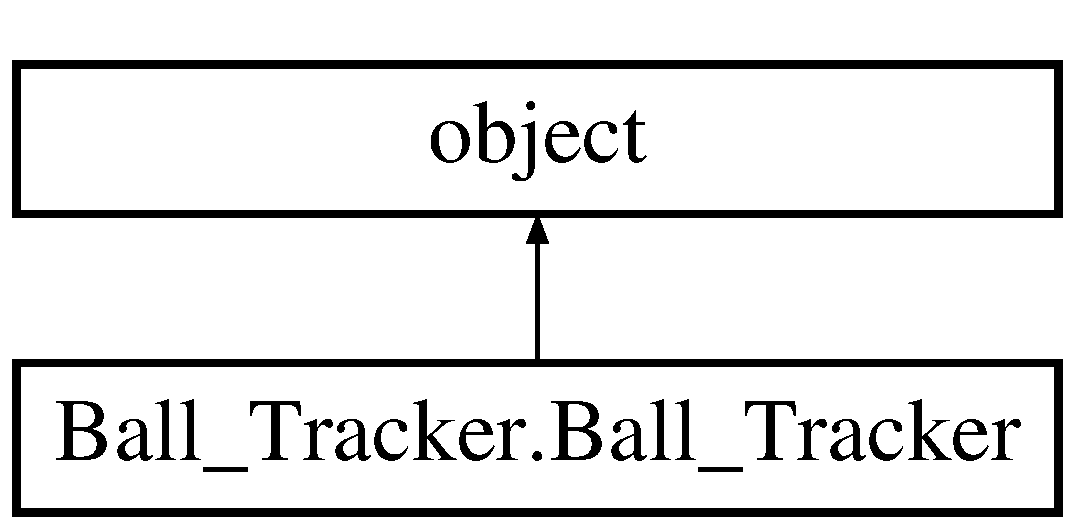
\includegraphics[height=2.000000cm]{classBall__Tracker_1_1Ball__Tracker}
\end{center}
\end{figure}
\subsection*{Public Member Functions}
\begin{DoxyCompactItemize}
\item 
def \hyperlink{classBall__Tracker_1_1Ball__Tracker_a9f52b5e12bec7868ae835e57cb4a2eb4}{\+\_\+\+\_\+init\+\_\+\+\_\+} (self, window\+Name, capture)
\item 
def \hyperlink{classBall__Tracker_1_1Ball__Tracker_a836189dde622b6c508895dc113e4bbc1}{run} (self)
\item 
def \hyperlink{classBall__Tracker_1_1Ball__Tracker_a7defc81aec0000c97a325487dd57ee5c}{on\+Keypress} (self, keycode)
\end{DoxyCompactItemize}
\subsection*{Public Attributes}
\begin{DoxyCompactItemize}
\item 
\mbox{\Hypertarget{classBall__Tracker_1_1Ball__Tracker_a3845d70e848af0a54873b54758a40dbc}\label{classBall__Tracker_1_1Ball__Tracker_a3845d70e848af0a54873b54758a40dbc}} 
{\bfseries orange\+Lower}
\item 
\mbox{\Hypertarget{classBall__Tracker_1_1Ball__Tracker_a435ac75c122115cc1c10a1eb551327d2}\label{classBall__Tracker_1_1Ball__Tracker_a435ac75c122115cc1c10a1eb551327d2}} 
{\bfseries orange\+Upper}
\item 
\mbox{\Hypertarget{classBall__Tracker_1_1Ball__Tracker_a4500869aebdcc924509e6c0832d2c8af}\label{classBall__Tracker_1_1Ball__Tracker_a4500869aebdcc924509e6c0832d2c8af}} 
{\bfseries points}
\end{DoxyCompactItemize}


\subsection{Constructor \& Destructor Documentation}
\mbox{\Hypertarget{classBall__Tracker_1_1Ball__Tracker_a9f52b5e12bec7868ae835e57cb4a2eb4}\label{classBall__Tracker_1_1Ball__Tracker_a9f52b5e12bec7868ae835e57cb4a2eb4}} 
\index{Ball\+\_\+\+Tracker\+::\+Ball\+\_\+\+Tracker@{Ball\+\_\+\+Tracker\+::\+Ball\+\_\+\+Tracker}!\+\_\+\+\_\+init\+\_\+\+\_\+@{\+\_\+\+\_\+init\+\_\+\+\_\+}}
\index{\+\_\+\+\_\+init\+\_\+\+\_\+@{\+\_\+\+\_\+init\+\_\+\+\_\+}!Ball\+\_\+\+Tracker\+::\+Ball\+\_\+\+Tracker@{Ball\+\_\+\+Tracker\+::\+Ball\+\_\+\+Tracker}}
\subsubsection{\texorpdfstring{\+\_\+\+\_\+init\+\_\+\+\_\+()}{\_\_init\_\_()}}
{\footnotesize\ttfamily def Ball\+\_\+\+Tracker.\+Ball\+\_\+\+Tracker.\+\_\+\+\_\+init\+\_\+\+\_\+ (\begin{DoxyParamCaption}\item[{}]{self,  }\item[{}]{window\+Name,  }\item[{}]{capture }\end{DoxyParamCaption})}

\begin{DoxyVerb}Constructor used to initialize the window manager, capture manager and ball detector
Also initializes orangeLower and orangeUpper which is a range of orange values used to help with detection
\end{DoxyVerb}
 

\subsection{Member Function Documentation}
\mbox{\Hypertarget{classBall__Tracker_1_1Ball__Tracker_a7defc81aec0000c97a325487dd57ee5c}\label{classBall__Tracker_1_1Ball__Tracker_a7defc81aec0000c97a325487dd57ee5c}} 
\index{Ball\+\_\+\+Tracker\+::\+Ball\+\_\+\+Tracker@{Ball\+\_\+\+Tracker\+::\+Ball\+\_\+\+Tracker}!on\+Keypress@{on\+Keypress}}
\index{on\+Keypress@{on\+Keypress}!Ball\+\_\+\+Tracker\+::\+Ball\+\_\+\+Tracker@{Ball\+\_\+\+Tracker\+::\+Ball\+\_\+\+Tracker}}
\subsubsection{\texorpdfstring{on\+Keypress()}{onKeypress()}}
{\footnotesize\ttfamily def Ball\+\_\+\+Tracker.\+Ball\+\_\+\+Tracker.\+on\+Keypress (\begin{DoxyParamCaption}\item[{}]{self,  }\item[{}]{keycode }\end{DoxyParamCaption})}

\begin{DoxyVerb}    Handle a keypress

    space -> Take a screenshot
    tab -> start / stop recording a screencast
    esc -> quit
\end{DoxyVerb}
 \mbox{\Hypertarget{classBall__Tracker_1_1Ball__Tracker_a836189dde622b6c508895dc113e4bbc1}\label{classBall__Tracker_1_1Ball__Tracker_a836189dde622b6c508895dc113e4bbc1}} 
\index{Ball\+\_\+\+Tracker\+::\+Ball\+\_\+\+Tracker@{Ball\+\_\+\+Tracker\+::\+Ball\+\_\+\+Tracker}!run@{run}}
\index{run@{run}!Ball\+\_\+\+Tracker\+::\+Ball\+\_\+\+Tracker@{Ball\+\_\+\+Tracker\+::\+Ball\+\_\+\+Tracker}}
\subsubsection{\texorpdfstring{run()}{run()}}
{\footnotesize\ttfamily def Ball\+\_\+\+Tracker.\+Ball\+\_\+\+Tracker.\+run (\begin{DoxyParamCaption}\item[{}]{self }\end{DoxyParamCaption})}

\begin{DoxyVerb}Runs the main application. It performs the following actions:

1. Initializes variables to store the current ball direction amount, the angles and the max height
2. Sets up meanshift tracking for the basketball
3. Computes end points of small line to check which direction the ball is moving.
4. Computes angle between points.
5. Computes the highest point reached.
6. Computes the highest point reached.
7. Continues to update the values frame by frame while the application is still running.
8. Returns the entry Angle, maximum ball height and exit angle if found.
9. Displays the corresponding values on screen.
\end{DoxyVerb}
 

The documentation for this class was generated from the following file\+:\begin{DoxyCompactItemize}
\item 
Ball\+\_\+\+Tracker.\+py\end{DoxyCompactItemize}

%--- End generated contents ---

% Index
\backmatter
\newpage
\phantomsection
\clearemptydoublepage
\addcontentsline{toc}{chapter}{Index}
\printindex

\end{document}
